% Auto-generated by figures/gen_latex_includes.py
% Copy snippets into the LaTeX manuscript after converting paper.md.

\begin{figure}[t]
    \centering
    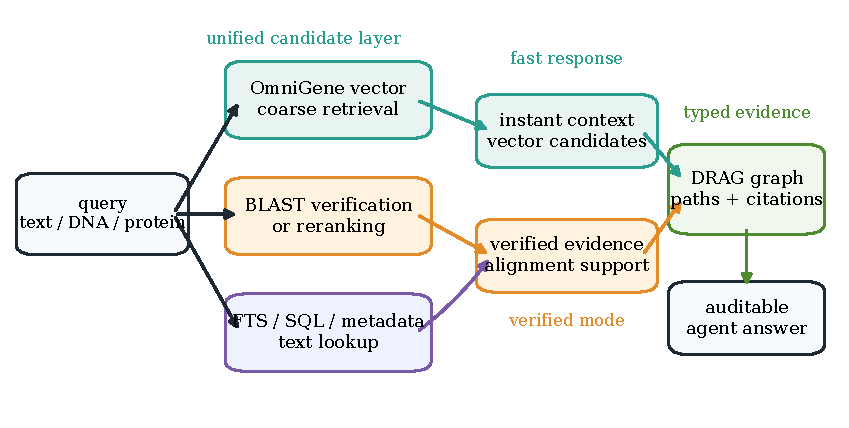
\includegraphics[width=0.95\textwidth]{figures/fig1_architecture.pdf}
    \caption{BioRAG-DRAG architecture. Vector retrieval provides an instant multimodal candidate layer; BLAST supplies sequence verification and reranking; DRAG packages vector, alignment, text, and graph evidence into typed traces for a local biomedical agent.}
    \label{fig:architecture}
\end{figure}

\begin{figure}[t]
    \centering
    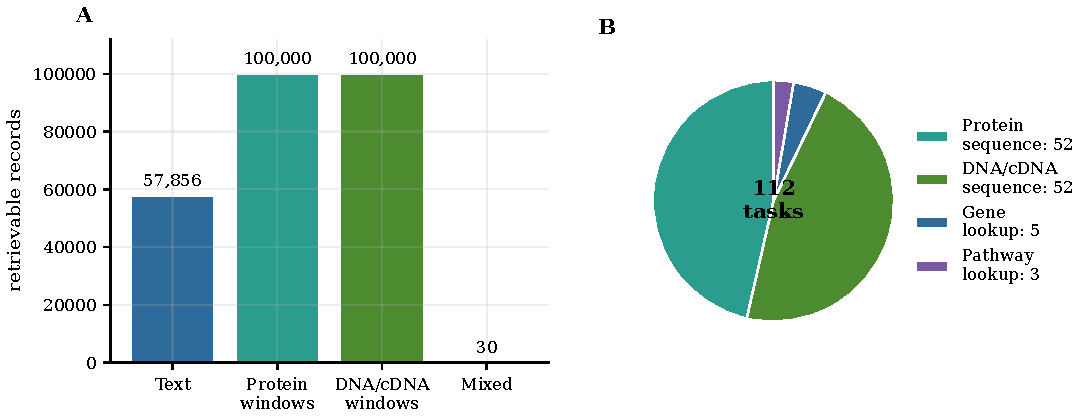
\includegraphics[width=0.95\textwidth]{figures/fig2_dataset.pdf}
    \caption{BioRAG-Standard v0 composition. The benchmark/library contains 257,886 retrievable records across Standard text, protein windows, DNA/cDNA windows, and mixed records, with 112 annotated retrieval tasks.}
    \label{fig:dataset}
\end{figure}

\begin{figure}[t]
    \centering
    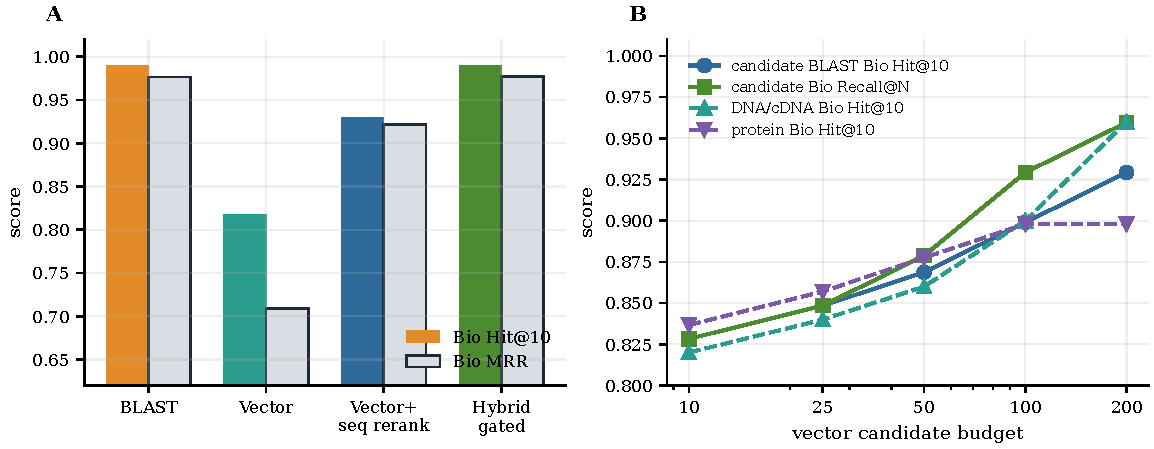
\includegraphics[width=0.95\textwidth]{figures/fig3_retrieval_quality.pdf}
    \caption{Retrieval quality on the 100-query sequence subset. BLAST remains the strongest alignment-grounded verifier, while vector retrieval provides useful candidate pools; candidate BLAST improves as the vector overfetch budget increases.}
    \label{fig:retrieval}
\end{figure}

\begin{figure}[t]
    \centering
    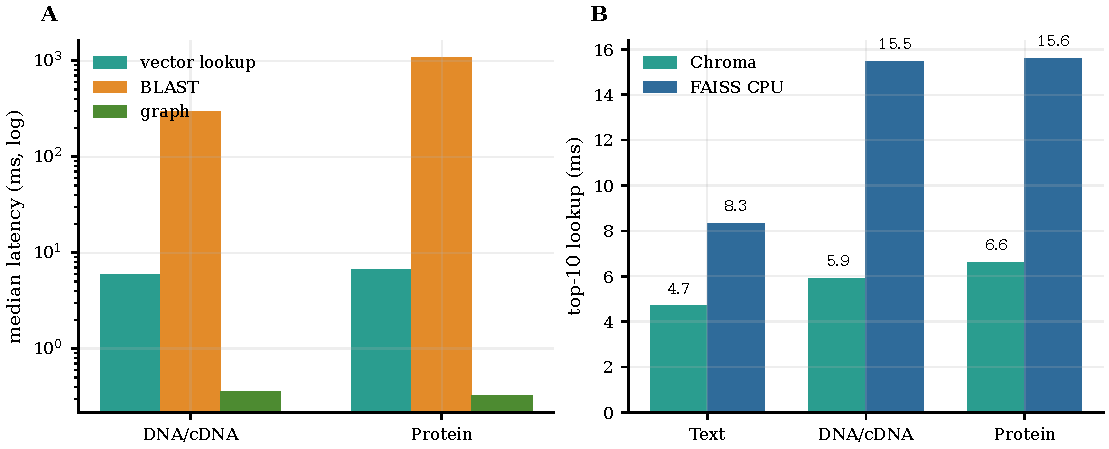
\includegraphics[width=0.95\textwidth]{figures/fig4_latency.pdf}
    \caption{Instant and verified retrieval latency. Vector lookup is measured after query embedding and supports an instant mode; BLAST dominates verified-mode latency, while graph expansion is negligible.}
    \label{fig:latency}
\end{figure}

\begin{figure}[t]
    \centering
    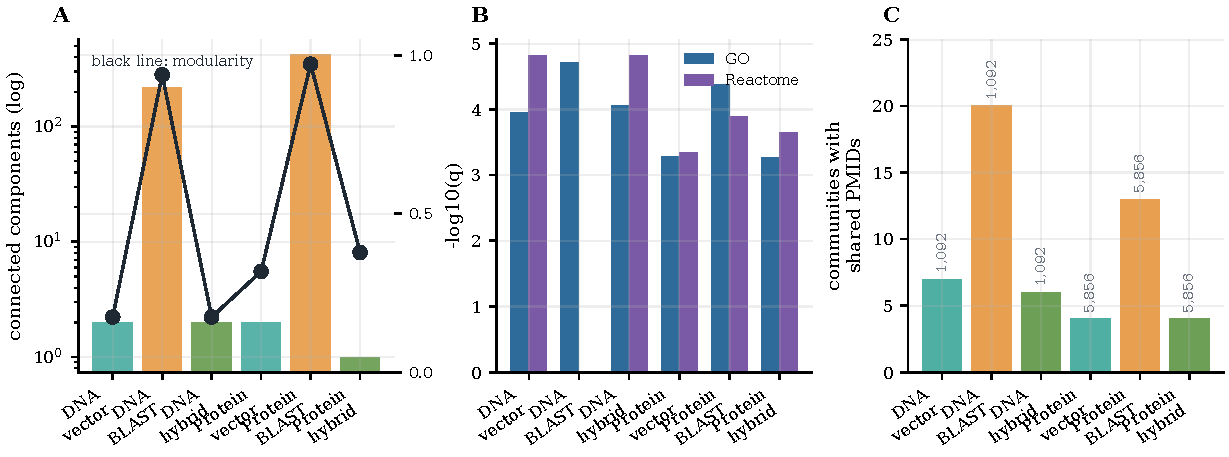
\includegraphics[width=0.95\textwidth]{figures/fig5_drag_biology.pdf}
    \caption{DRAG biological-structure analysis. Vector, BLAST, and hybrid graphs expose different graph connectivity, functional enrichment, and literature-sharing patterns; these signals support hypothesis-generating biological evidence organization.}
    \label{fig:drag_biology}
\end{figure}
